% !TeX root = ../../../book.tex
\subsection{证明 ``$\subseteq$''}

回想一下子集的定义,因为接下来我们会频繁使用它:

\begin{definition}
    给定两个集合 $A$ 和 $B$,如果 $A$ 的每个元素也是 $B$ 的元素,那么我们说 $A$ 是 $B$ 的\dotuline{子集}。
\end{definition}

假设我们遇到如下问题:
\begin{center}
    设 $A$ 为集合…… 并设 $B$ 为集合…… 证明 $A \subseteq B$。
\end{center}
我们如何利用 $A \subseteq B$ 的定义来证明这个主张?是的,直观的想法是``$A$ 的每个元素也是 $B$ 的元素'',但我们不应该只是试图绕过这个问题而将这句话作为我们的结论。相反,我们需要验证 $A$ 的每个元素也必然是 $B$ 的元素。这就是``\textbf{任意固定}'' 这句美妙的短语派上用场的地方!

\subsubsection*{``任意固定''}

我们怎样才能同时讨论 $A$ 的\emph{所有可能元素}呢?当然,如果 $A$ 只有 $3$ 个元素,我们可能只需一一检查即可。但是如果 $A$ 有 $100$ 个元素怎么办?如果有 $100$ 万个元素呢?甚至\emph{无穷}多个呢?我们怎样才能以合理的方式同时证明所有这些元素呢?

我们要做的就是引入 $A$ 的\textbf{任意固定}元素,这样我们就有了可以使用的东西。这个元素是\textbf{任意的},因为我们不对它是什么或它具有什么属性做任何额外的假设,只要它是 $A$ 的元素即可。这个元素是\textbf{固定的},因为我们将为其分配某个变量名(通常是一个字母,例如 $a$ 或 $x$ 或 $t$ 等),并且该字母在我们证明的其余部分中代表\emph{相同的}对象。只要我们能证明这个元素满足目标,那么我们就同时证明了 $A$ 的\emph{所有}元素。

\subsubsection*{示例}

让我们看看这个过程的实际应用,以真正理解这一点。我们将从要证明的陈述开始,接着描述提出证明的思维过程,然后给出正式的书面证明。

\begin{lemma}\label{lemma3.9.1}
    设 $A,B,X$ 为任意集合。如果 $X \subseteq A$ 且 $X \subseteq B$, 则 $X \subseteq A \cap B$。
\end{lemma}

\emph{直觉}:考虑绘制维恩(Venn)图来表示这种情况。为了确保 $X \subseteq A$ 和 $X \subseteq B$ 同时成立,我们需要令集合 $X$ 位于 $A$ 和 $B$ 的``内部''。相应地,这意味着 $X$ 必须完全位于 $A$ 和 $B$ 重叠的``内部'',即 $A \cap B$ 代表的部分。这有助于我们认识到这个说法确实是正确的。但这并不构成证明!
\begin{center}
    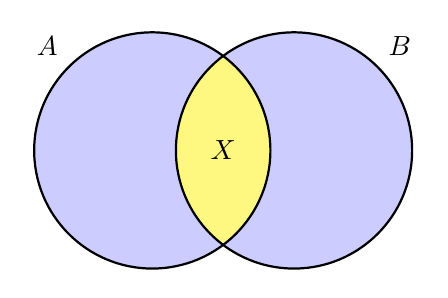
\begin{tikzpicture}[thick, set/.style = {circle, minimum size = 3cm, fill=blue!20}]

        % Set A
        \node[set,label={135:$A$}] (A) at (0,0) {};

        % Set B
        \node[set,label={45:$B$}] (B) at (1.8,0) {};

        % Intersection
        \begin{scope}
            \clip (0,0) circle(1.5cm);
            \clip (1.8,0) circle(1.5cm);
            \fill[yellow!50](0,0) circle(1.5cm);
        \end{scope}

        % Circles outline
        \draw (0,0) circle(1.5cm);
        \draw (1.8,0) circle(1.5cm);

        % Set intersection label
        \node at (0.9,0) {$X$};
    \end{tikzpicture} 
\end{center}

为了\emph{证明}这个命题,我们将引入任意固定的元素 $x \in X$。我们对它了解多少呢?我们假设 $X \subseteq A$。``$\subseteq$'' 的定义意味着 $X$ 的所有元素也是 $A$ 的元素。现在我们知道 $x$ 是 $X$ 的元素;这意味着它也是 $A$ 的一个元素。多么方便啊!我们可以对 $x$ 和 $X$ 和 $B$ 做出一些类似的陈述,这将告诉我们 $x \in B$。综上,这意味着什么?我们发现可以用 ``$\cap$'' 的定义,这告诉我们 $x \in A \cap B$。太棒了!现在,我们把它写下来。

\begin{proof}
    设 $x \in X$ 为任意固定元素。

    假设 $X \subseteq A$,根据 $\subseteq$ 的定义,可得 $x \in A$。

    同理,假设 $X \subseteq B$,可得 $x \in B$。

    因为 $x \in A$ 且 $x \in B$,根据 $\cap$ 的定义,这意味着 $x \in A \cap B$。

    综上,我们证明了当 $x \in X$ 时,$x \in A \cap B$ 也成立。由于 $x \in X$ 是任意的,因此我们得出 $X \subseteq A \cap B$ 的结论。
\end{proof}

怎么样,还不错吧?让我们看一个稍微复杂一点的例子。

\begin{proposition}
    设 $A$ 和 $B$ 为任意集合。则 $\mathcal{P}(A) \cap \mathcal{P}(B) \subseteq \mathcal{P}(A \cap B)$。
\end{proposition}

哇,这是真的吗? 回顾 \ref{sec:section3.5} 节中的问题 \ref{exc:exercises3.5.6},你会看到一个具体例子。这表明,\emph{一般而言},这一说法是正确的,而不仅仅是针对该示例。让我们找出为什么这是正确的,并证明它。

\emph{直觉}:这里有几个层次的定义共同发挥作用。特别是,幂集运算可能会让你感到困惑。关键是记住这个定义:$\mathcal{P}(A)$ 是 $A$ 的所有子集的集合。现在,这里的主要主张是一个子集关系:无论集合 $\mathcal{P}(A) \cap \mathcal{P}(B)$ 是什么(我们稍后会对其进行分析,但眼下重要的是你要立即意识到到它是什么类型的对象:集合),它应该是集合 $\mathcal{P}(A \cap B)$ 的子集。值得注意的是,这确实激发了即将到来的证明的总体形式。

甚至无需考虑 $\mathcal{P}(A) \cap \mathcal{P}(B)$ 的含义,我们就可以确定我们的证明将从``令 $X \in \mathcal{P}(A) \cap \mathcal{P}(B)$ 为任意固定集合''开始。这是因为我们需要通过获取左侧集合中的任意元素并推断它也是右侧集合中的元素来满足``$\subseteq$''的定义。这就是我们所说的证明的\textbf{结构}。

元素 $X \in \mathcal{P}(A) \cap \mathcal{P}(B)$ ``看起来像什么''?它是一个集合,并且是 $P(A)$ 和 $P(B)$ 的元素。这意味着……好吧,实际上我们现在要直接跳到正式证明,因为无论如何我们都会发现自己在下面重复相同的单词。但在继续阅读我们的证明之前,我们认为你应该尝试编写自己的证明。做完之后,你可以对比一下,看看你的做法是否正确,是不是和我们的步骤一样,写的是否清楚等等。看看你能做到什么程度!

\begin{proof}
    设 $X \in \mathcal{P}(A) \cap \mathcal{P}(B)$ 为任意固定集合。

    根据 $\cap$ 的定义,这意味着 $X \in \mathcal{P}(A)$ 且 $X \in \mathcal{P}(B)$。

    因为 $X \in \mathcal{P}(A)$,根据幂集的定义,我们知道 $X \subseteq A$。

    同理,因为 $X \in \mathcal{P}(B)$,我们知道 $X \subseteq B$。

    因为 $X \subseteq A$ 且 $X \subseteq B$,根据我们刚刚证明的引理 \ref{lemma3.9.1},可得 $X \subseteq A \cap B$。

    因为 $X \subseteq A \cap B$,根据幂集的定义,我们知道 $X \in \mathcal{P}(A \cap B)$。

    因为 $X$ 是任意固定集合,因此我们得出结论 $\mathcal{P}(A) \cap \mathcal{P}(B) \subseteq \mathcal{P}(A \cap B)$。
\end{proof}

你的证法跟上面的一样吗?你也引用了前面的引理吗?你是否在没有意识到的情况下再次证明了这个结果?把它当作一个教训!证明结果的主要好处之一是我们可以在以后的证明中使用它们!在一个证明过程中再次证明之前的结果在技术上并没有什么问题;但不重复证明会节省一点时间。如果你发现自己正在解决一个问题并发觉:“嘿,这感觉很熟悉……”,回去寻找相关的定理或引理或例子。也许你可以利用一些已经获得的知识来发挥自己的优势。
